\documentclass{physlab}
\usepackage{ctable}

%\newenvironment{bottompar}{\par\vspace*{\fill}}{\clearpage}

\begin{document}
	\begin{titlepage}
\center % Center everything on the page
 
%----------------------------------------------------------------------------------------
%	HEADING SECTIONS
%----------------------------------------------------------------------------------------

\textsc{\LARGE Московский\\[-0.2cm]Физико-Технический Институт\\[0.1cm]\large (государственный университет)}\\[1.5cm] % Name of your university/college
\textsc{\Large Кафедра общей физики}\\[0.1cm] % Major heading such as course name
\textsc{\large Лабораторная работа № 123}\\[0.5cm] % Minor heading such as course title

%----------------------------------------------------------------------------------------
%	TITLE SECTION
%----------------------------------------------------------------------------------------

\HRule
\\[0.6cm]
{ \huge \bfseries Резонанс токов.}
\\[0.3cm] % Title of your document
\HRule
\\[1.5cm]


 
%----------------------------------------------------------------------------------------
%	AUTHOR SECTION
%----------------------------------------------------------------------------------------

	\begin{minipage}{0.4\textwidth}
	\begin{flushleft} \large
		\emph{Автор:}\\
		Алексей \textsc{Домрачев} \\
		615 группа
	\end{flushleft}
\end{minipage}
~
\begin{minipage}{0.4\textwidth}
	\begin{flushright} \large
		\emph{Преподаватель:} \\
		Николай Владимирович \textsc{Дьячков} % Supervisor's Name
	\end{flushright}
\end{minipage}

\begin{bottompar}
	\begin{center}
		
\includegraphics[width = 80 mm]{logo.jpg}
	\end{center}
	{\large \today}
	
\end{bottompar}
\vfill % Fill the rest of the page with whitespace
\end{titlepage}


\paragraph{Цель работы.} Исследование резонанса токов в параллельном колебательном контуре с изменяемой ёмкостью, включающее получение АЧХ и ФЧХ, а также определение основных параметров контура.

\paragraph{В работе используются:} генератор сигналов, источник тока, нагруженный на параллельный колебательный контур с переменной ёмкостью, двулучевой осциллограф, цифровые вольтметры.

\paragraph{Установка и краткая теория.} Схема экспериментального стенда для изучения резонанса токов в параллельном колебательном контуре показана на рис. \ref{ris:image1}~a, на рис. \ref{ris:image1}~б контур представлен почти в натуральную величину.
\begin{figure}[H]
	\begin{minipage}[H]{0.49\linewidth}
		\center{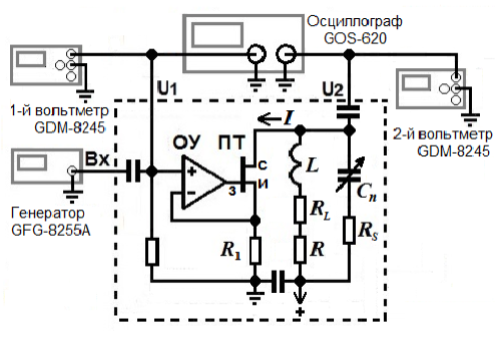
\includegraphics[width=80mm]{aparatus1} \\ а)}
	\end{minipage}
	\hfill
	\begin{minipage}[h]{0.49\linewidth}
		\center{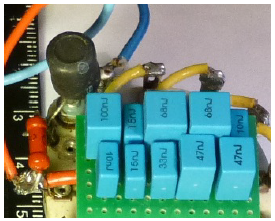
\includegraphics[width=80mm]{aparatus2} \\ б)}
	\end{minipage}
	\caption{Экспериментальная установка.}
	\label{ris:image1}
\end{figure}
Выведем формулу для добротности:
\begin{equation}
U=Q\rho I\Rightarrow Q =\frac{U R_1}{\rho E_0}
\end{equation}
$R_\Sigma$ будет вычисляться по формуле, так как оно должно быть рассчитано при последовательном обходе контура:
\begin{equation}
	R_\Sigma=R_L+R+R_S
	\label{eq:Rsum}
\end{equation}
Из курса общей физики известно, что частота резонанса можно вычислить по формуле
\begin{equation}
	f_0=\frac{1}{2\pi \sqrt{LC}}
\end{equation}
Отсюда можно посчитать $L$:
\begin{equation}
	L=\frac{1}{4\pi C f_0^2}
	\label{eq:L}
\end{equation}
Для расчета $Z_\text{рез}$ понадобится вычислить волновое сопротивление:
\begin{equation}
	\rho = \sqrt{L/C}
	\label{eq:rho}
\end{equation}
Теперь можем рассчитать  $Z_\text{рез}$:
\begin{equation}
	Z_\text{рез}=\rho Q^2
	\label{eq:Q}
\end{equation}
Эквивалентное последовательное сопротивление связано с волновым соотношением:
\begin{equation}
	R_S=\rho\cdot 10^{-3}
	\label{eq:RS}
\end{equation}
\paragraph{Обработка и представление результатов.} Представим полученные и рассчитанные по формулам выше значения в таблице~\ref{table1}

\begin{table}[H]
	\centering
	\caption{Расчеты пункта 11}
	\label{table1}
	\begin{tabular}{c|c|c|c|c|c|c|c|c|c|c|c}
		\toprule
		$n$ & $C_n$, нФ & $f_{0n}$, кГц & $U$, В & $E$, В & $L$, мкГн & $\rho$, Ом & \begin{tabular}[c]{@{}c@{}}$Z_\text{рез}$,\\  Ом\end{tabular} & $Q$ & \begin{tabular}[c]{@{}c@{}}$R_\Sigma$,\\ Ом\end{tabular} & \begin{tabular}[c]{@{}c@{}}$R_\text{smax}$,\\ Ом\end{tabular} & \begin{tabular}[c]{@{}c@{}}$R_L$,\\  Ом\end{tabular} \\ \midrule
		1 & 25.1 & 32.1 & 1.12 & 0.185 & 979 & 198 & 178945 & 33.0 & 5.99 & 0.20 & 2.29\\
		2 & 33.2 & 27.8 & 0.91 & 0.186 & 987 & 172 & 134405 & 30.7 & 5.60 & 0.17 & 1.93 \\
		3 & 47.3 & 23.2 & 0.66 & 0.188 & 995 & 144 & 82602  & 26.3 & 5.48 & 0.14 & 1.84 \\
		4 & 57.4 & 21.2 & 0.55 & 0.188 & 982 & 131 & 63191  & 24.1 & 5.42 & 0.13 & 1.79 \\
		5 & 67.5 & 19.5 & 0.47 & 0.189 & 987 & 121 & 49512  & 22.3 & 5.42 & 0.12 & 1.80 \\
		6 & 82.7 & 17.7 & 0.39 & 0.189 & 978 & 109 & 37735  & 20.4 & 5.33 & 0.11 & 1.73 \\
		7 & 101.6 & 16.0 & 0.32 & 0.190 & 974 & 98 & 27863  & 18.5 & 5.32 & 0.10 & 1.72 \\ \bottomrule
	\end{tabular}
\end{table}
Сделаем несколько выводов из таблицы:
\begin{enumerate}
	\item $\left< L \right>$ = 983, $\Delta L=3$, случайная погрешность равна 0.23.
	\item  $\left< R_L \right>$ = 1.87, $\Delta R_L=0,08$, случайная погрешность равна 0.01.
\end{enumerate}
Построим и сравним графики АЧХ для $C_1$ и $C_7$ 
\begin{table}[H]
	\centering
	\caption{АЧХ для $C_1$}
	\label{table2.1}
	\begin{tabular}{c|c c c c c c c c}
		\toprule
		$f$, кГц & 31.30 & 31.40 & 31.55 & 31.64 & 31.80 & 32.46 & 32.50 & 32.66 \\ 
		$U$, В   & 0.67  & 0.67  & 0.78  & 0.85  & 0.99  & 0.94  & 0.89  & 0.78  \\ \bottomrule
	\end{tabular}
\end{table}
\begin{table}[H]
	\centering
	\caption{АЧХ для $C_7$}
	\label{table2.2}
	\begin{tabular}{c|c c c c c c c c}
		\toprule
		$f$, кГц & 15.10 & 15.30 & 15.61 & 15.83 & 16.01   & 16.32 & 16.80 & 16.90 \\ 
		$U$, В   & 0.14 & 0.17 & 0.24 & 0.28 & 0.32 & 0.28 & 0.17 & 0.16 \\ \bottomrule
	\end{tabular}
\end{table}

\begin{figure}[H]
	\begin{minipage}[H]{0.49\linewidth}
		\center{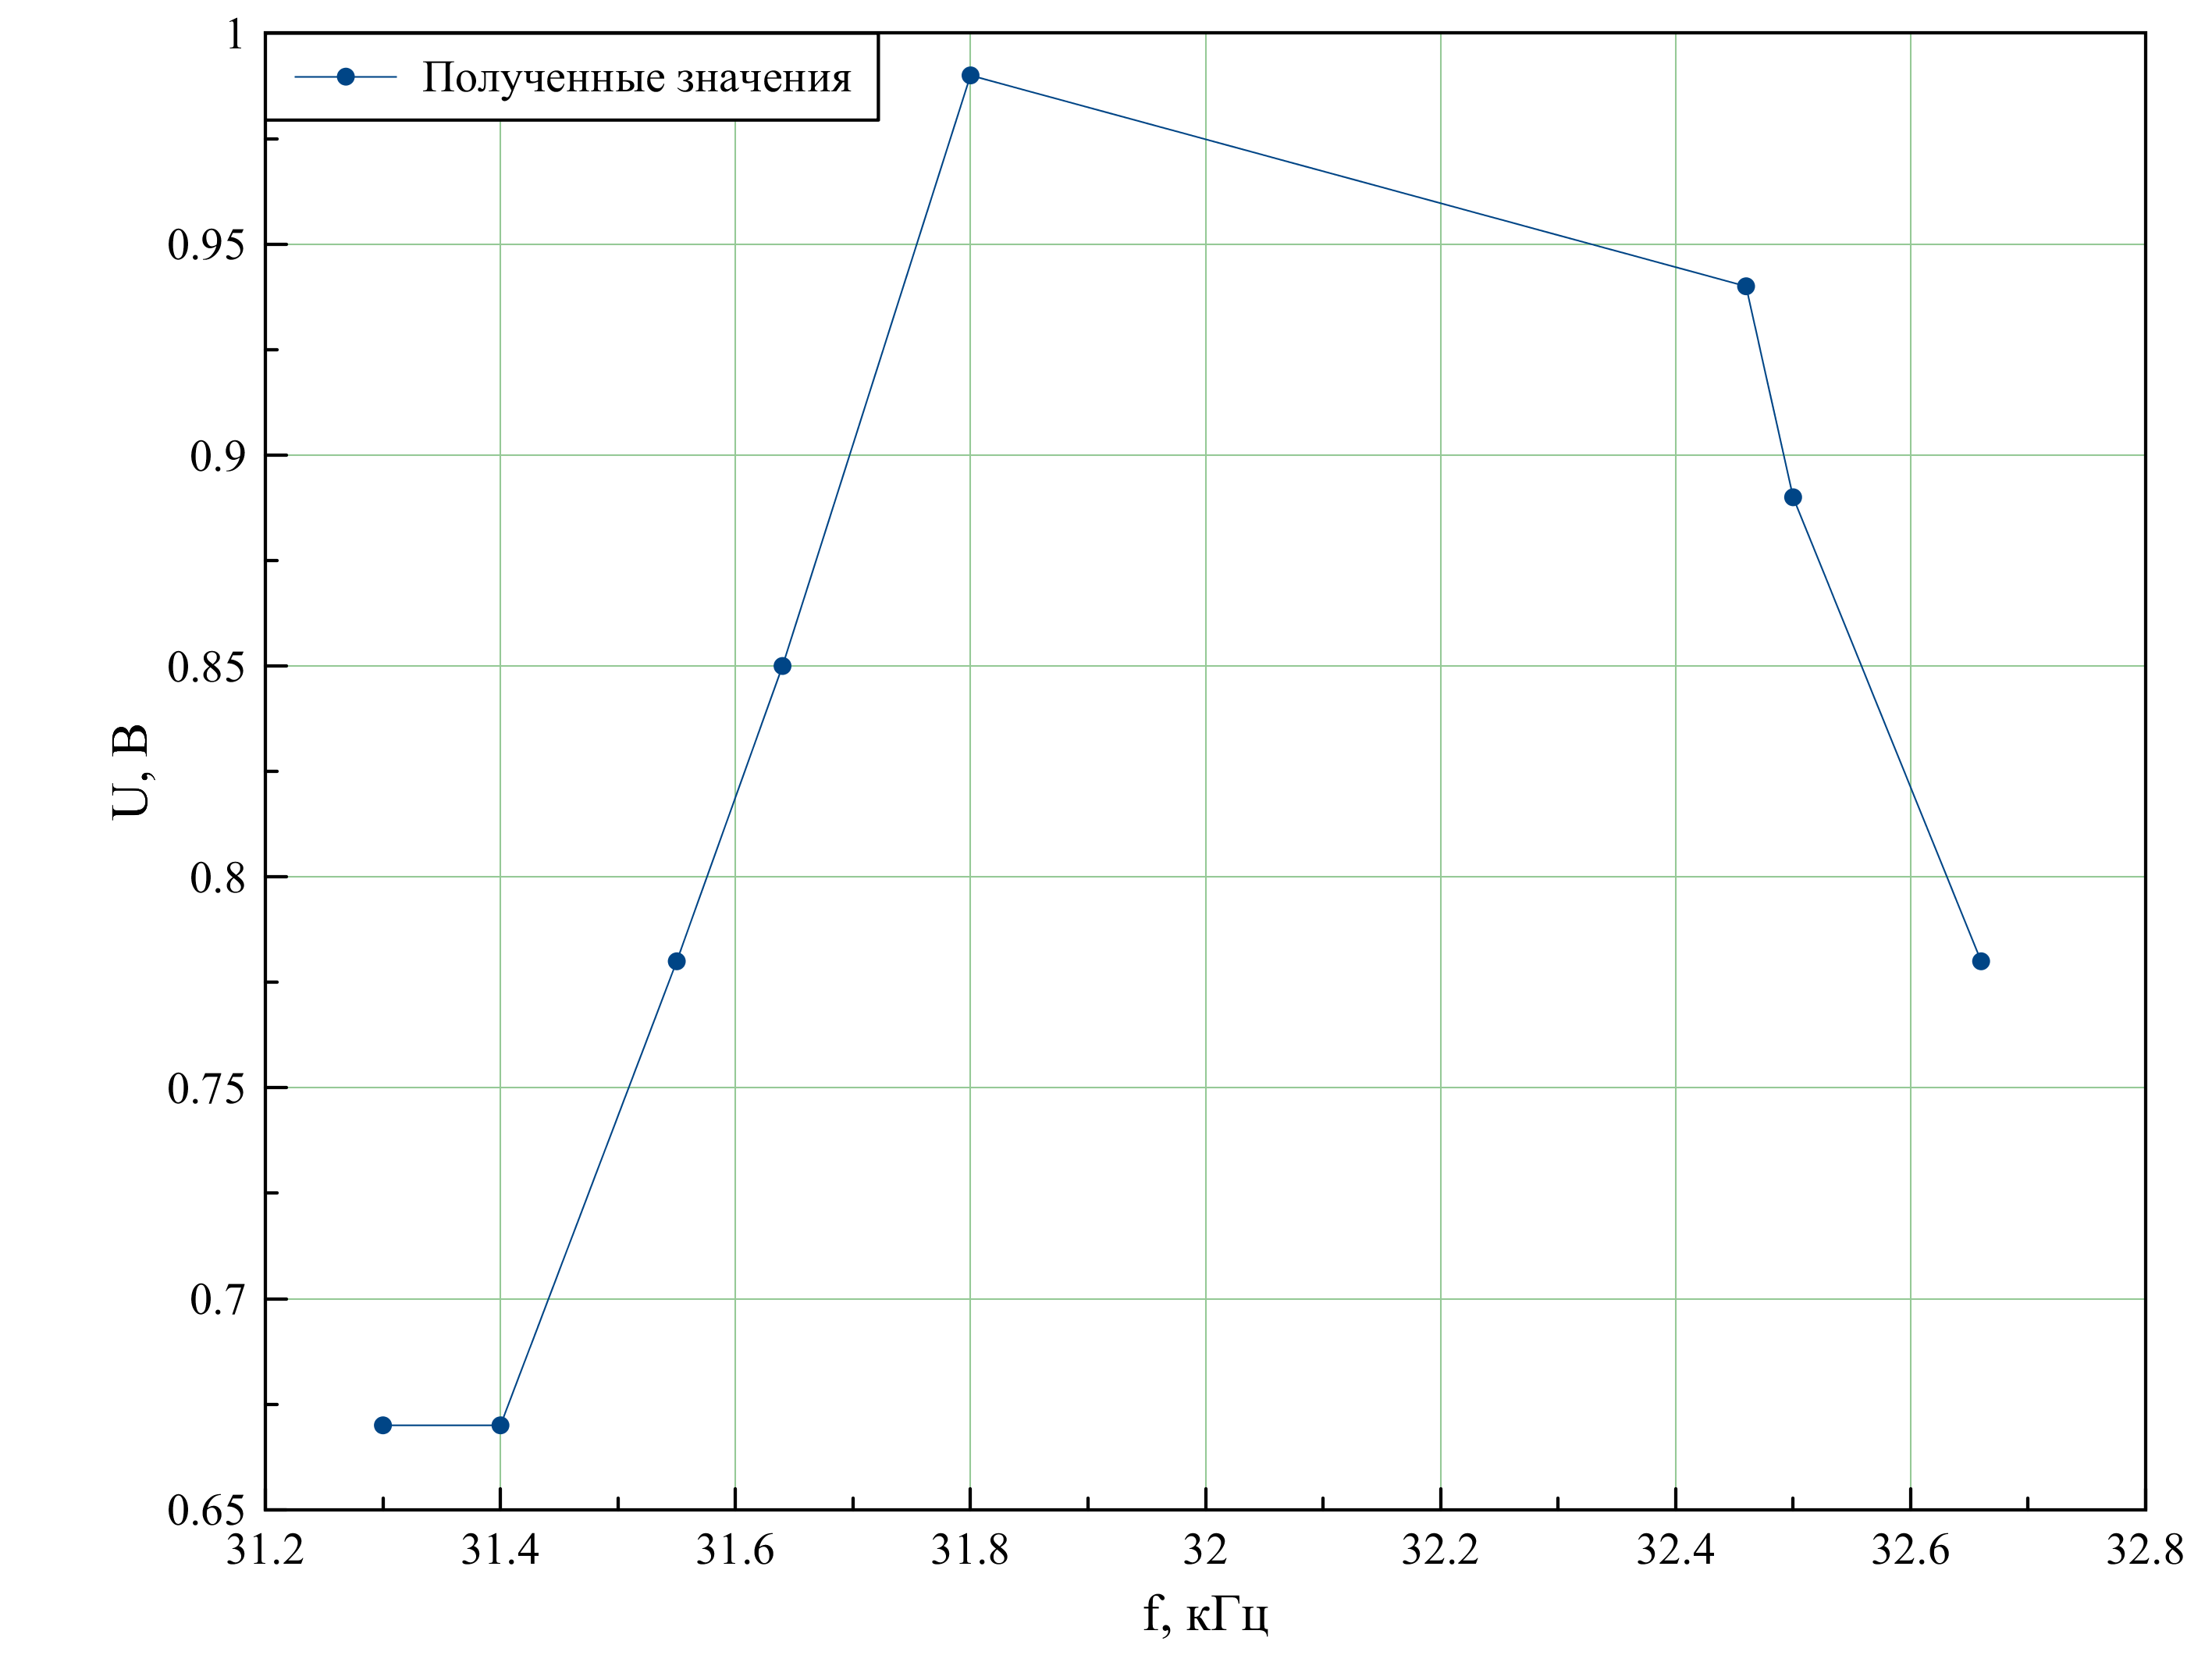
\includegraphics[width=85mm]{ACH_C1} \\ $C_1$}
	\end{minipage}
	~
	\begin{minipage}[h]{0.49\linewidth}
		\center{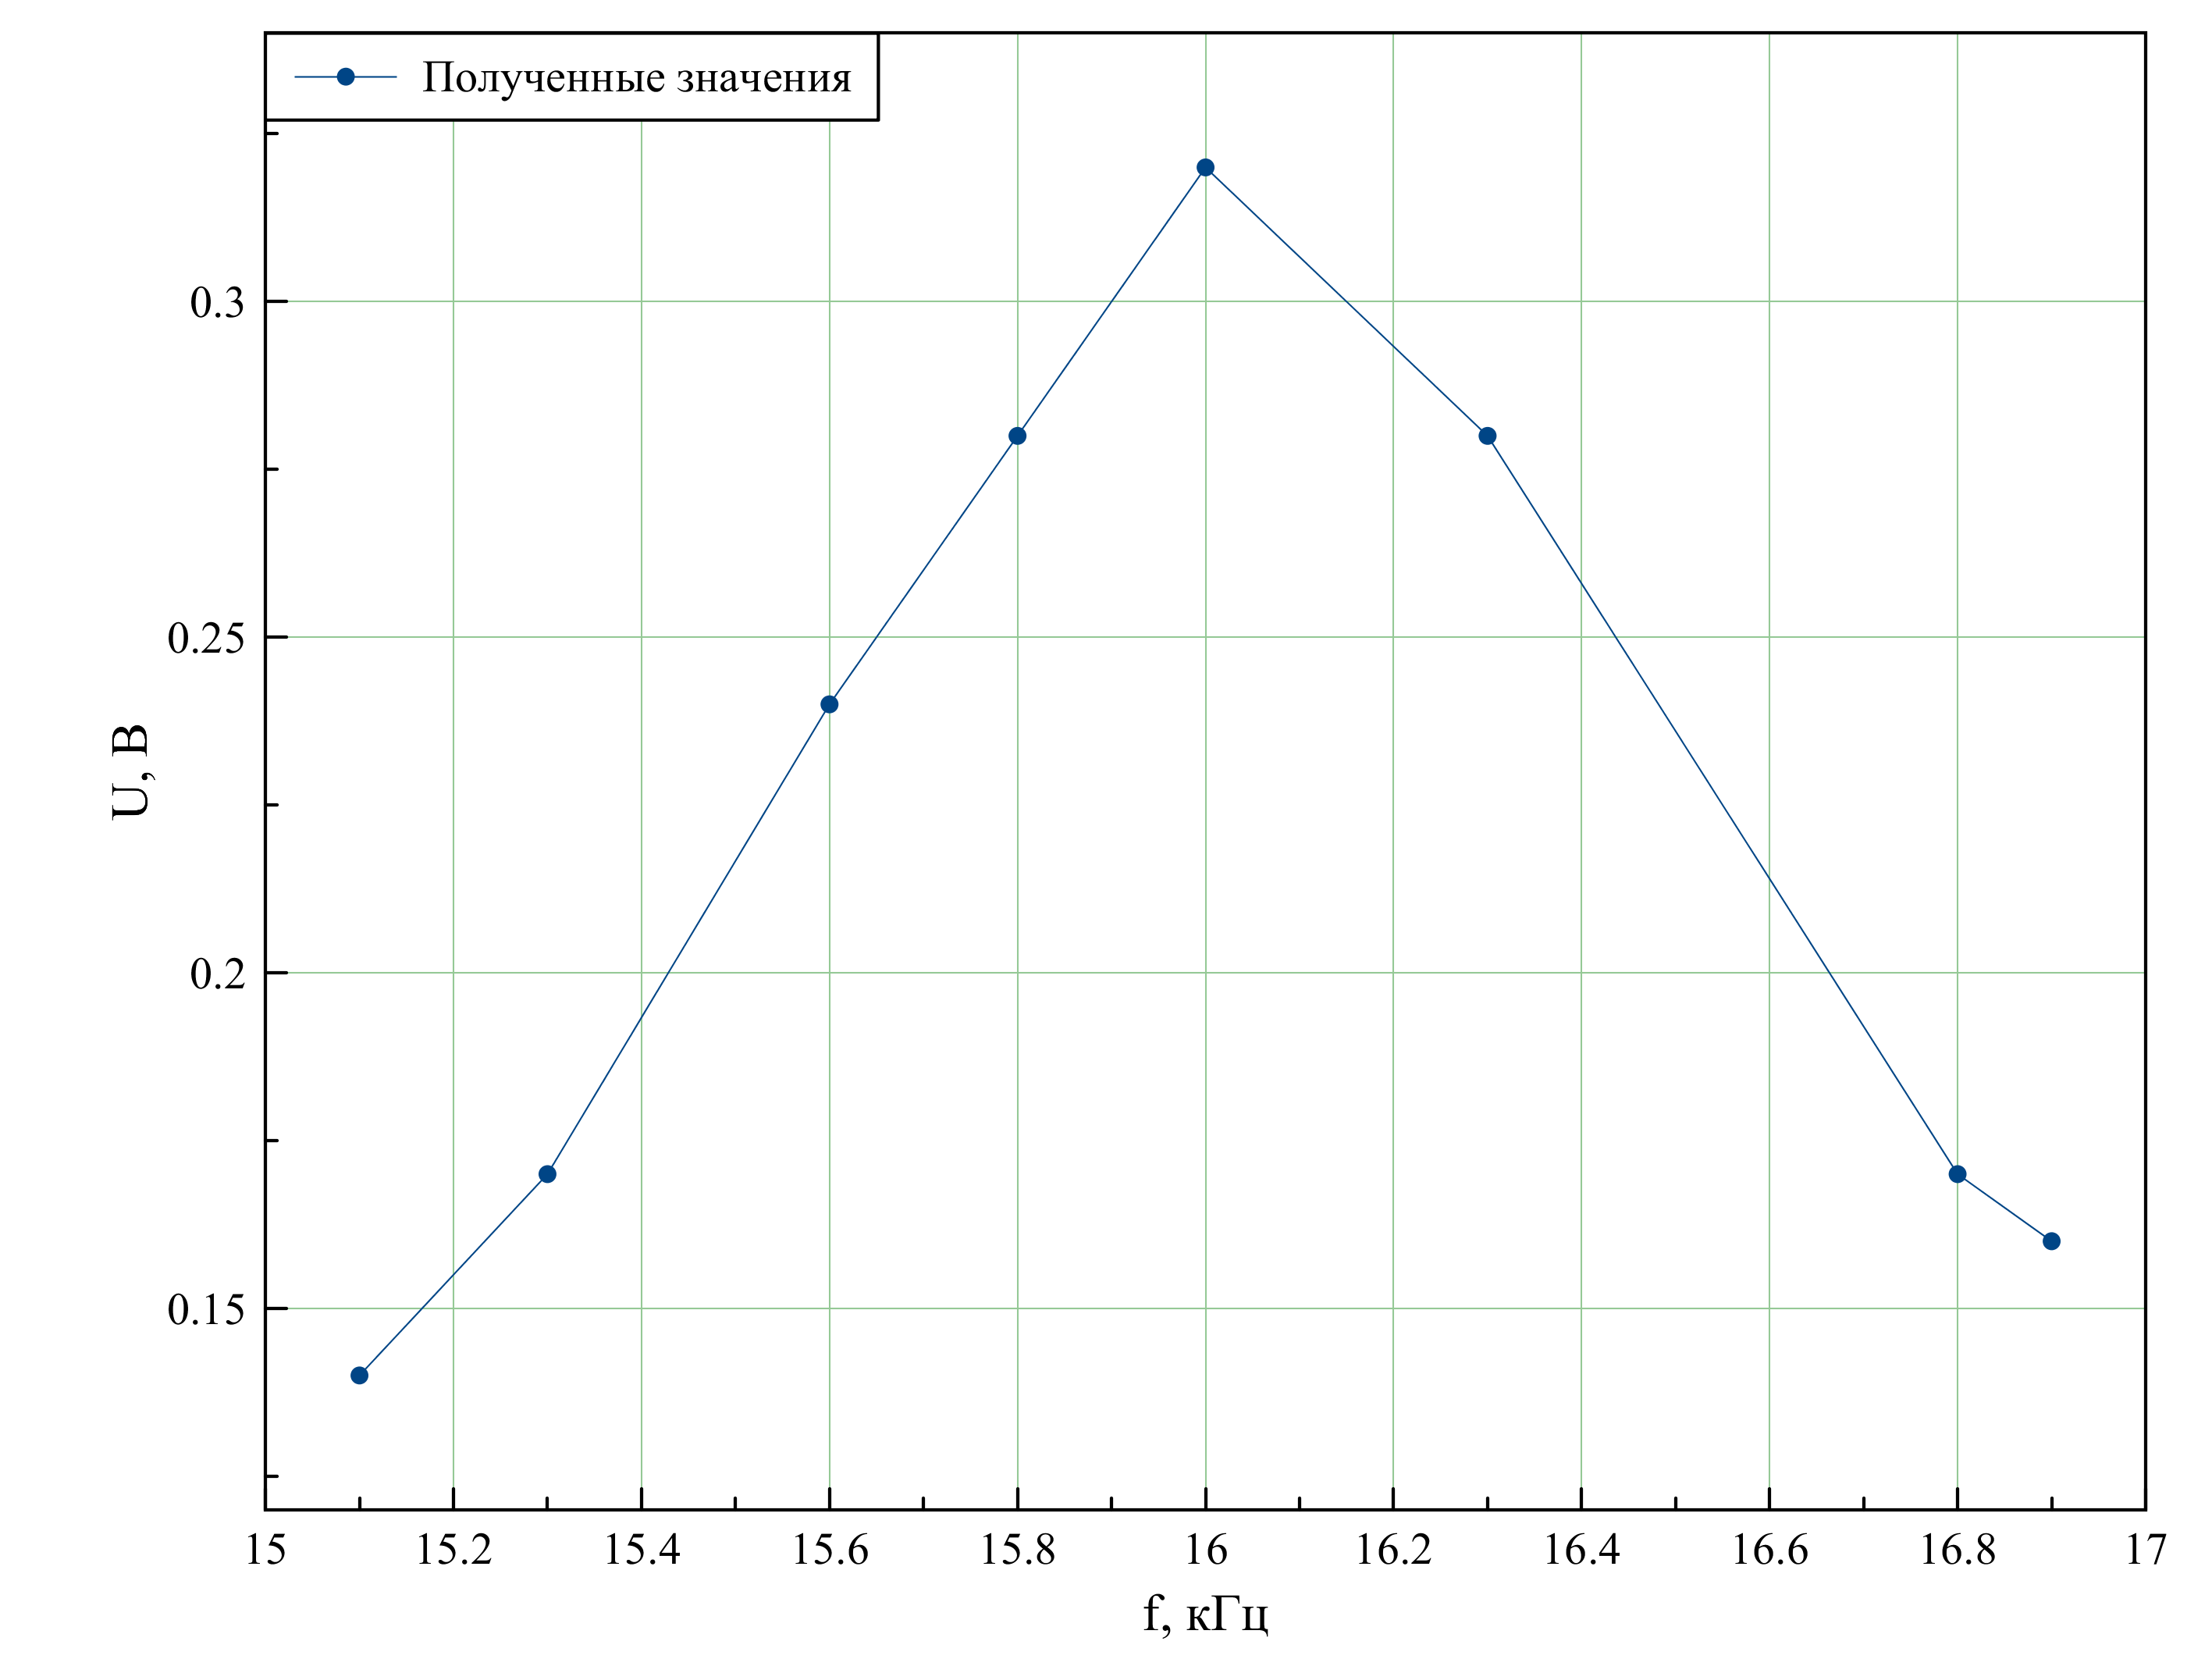
\includegraphics[width=85mm]{ACH_C7} \\ $C_7$}
	\end{minipage}
	\caption{Амплитудно-частотные характеристики.}
	\label{ris:image2}
\end{figure}
По графикам видно, что частоты, при которых достигается резонанс отличаются в два раза, а резонансные значения амплитуды примерно в 3 раза.

Также построим АЧХ в безразмерных координатах $x\equiv f/f_{0n},\;y \equiv U(x)/U(f_{0n})$, чтобы определить добротность.
\begin{figure}[H]
	\begin{minipage}[H]{0.49\linewidth}
		\center{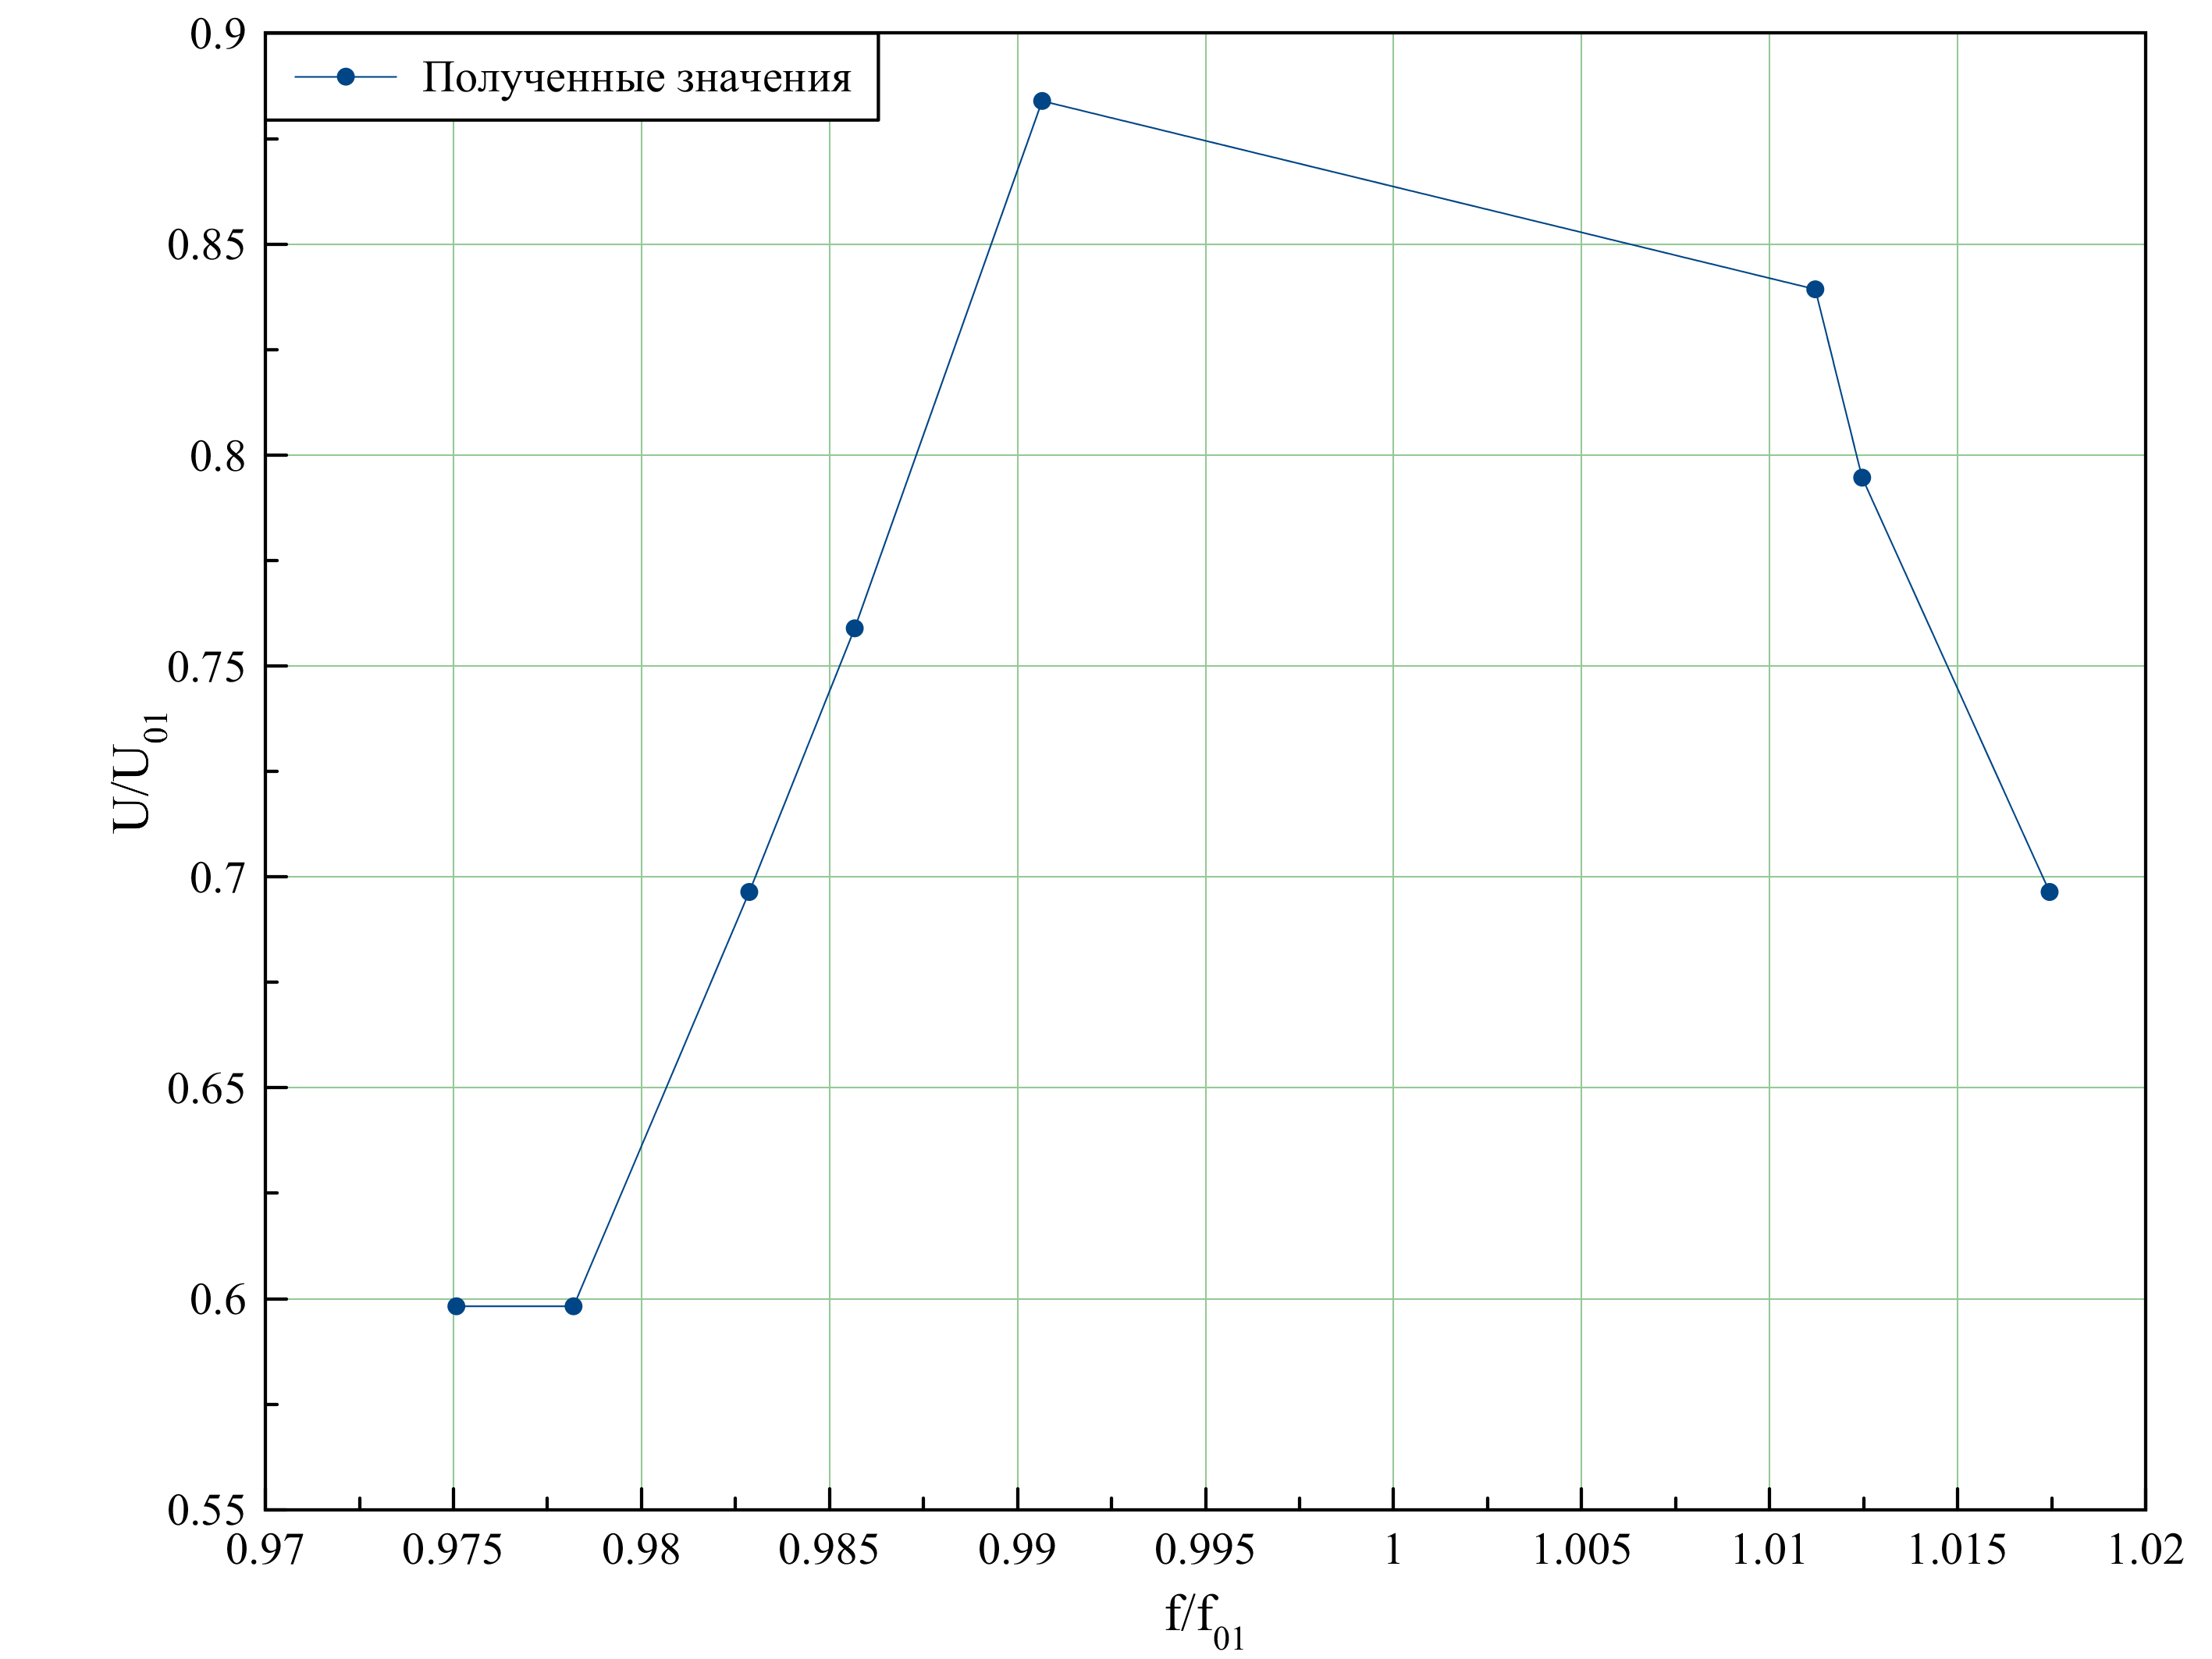
\includegraphics[width=85mm]{2ACH_C1} \\ $C_1$}
	\end{minipage}
	~
	\begin{minipage}[h]{0.49\linewidth}
		\center{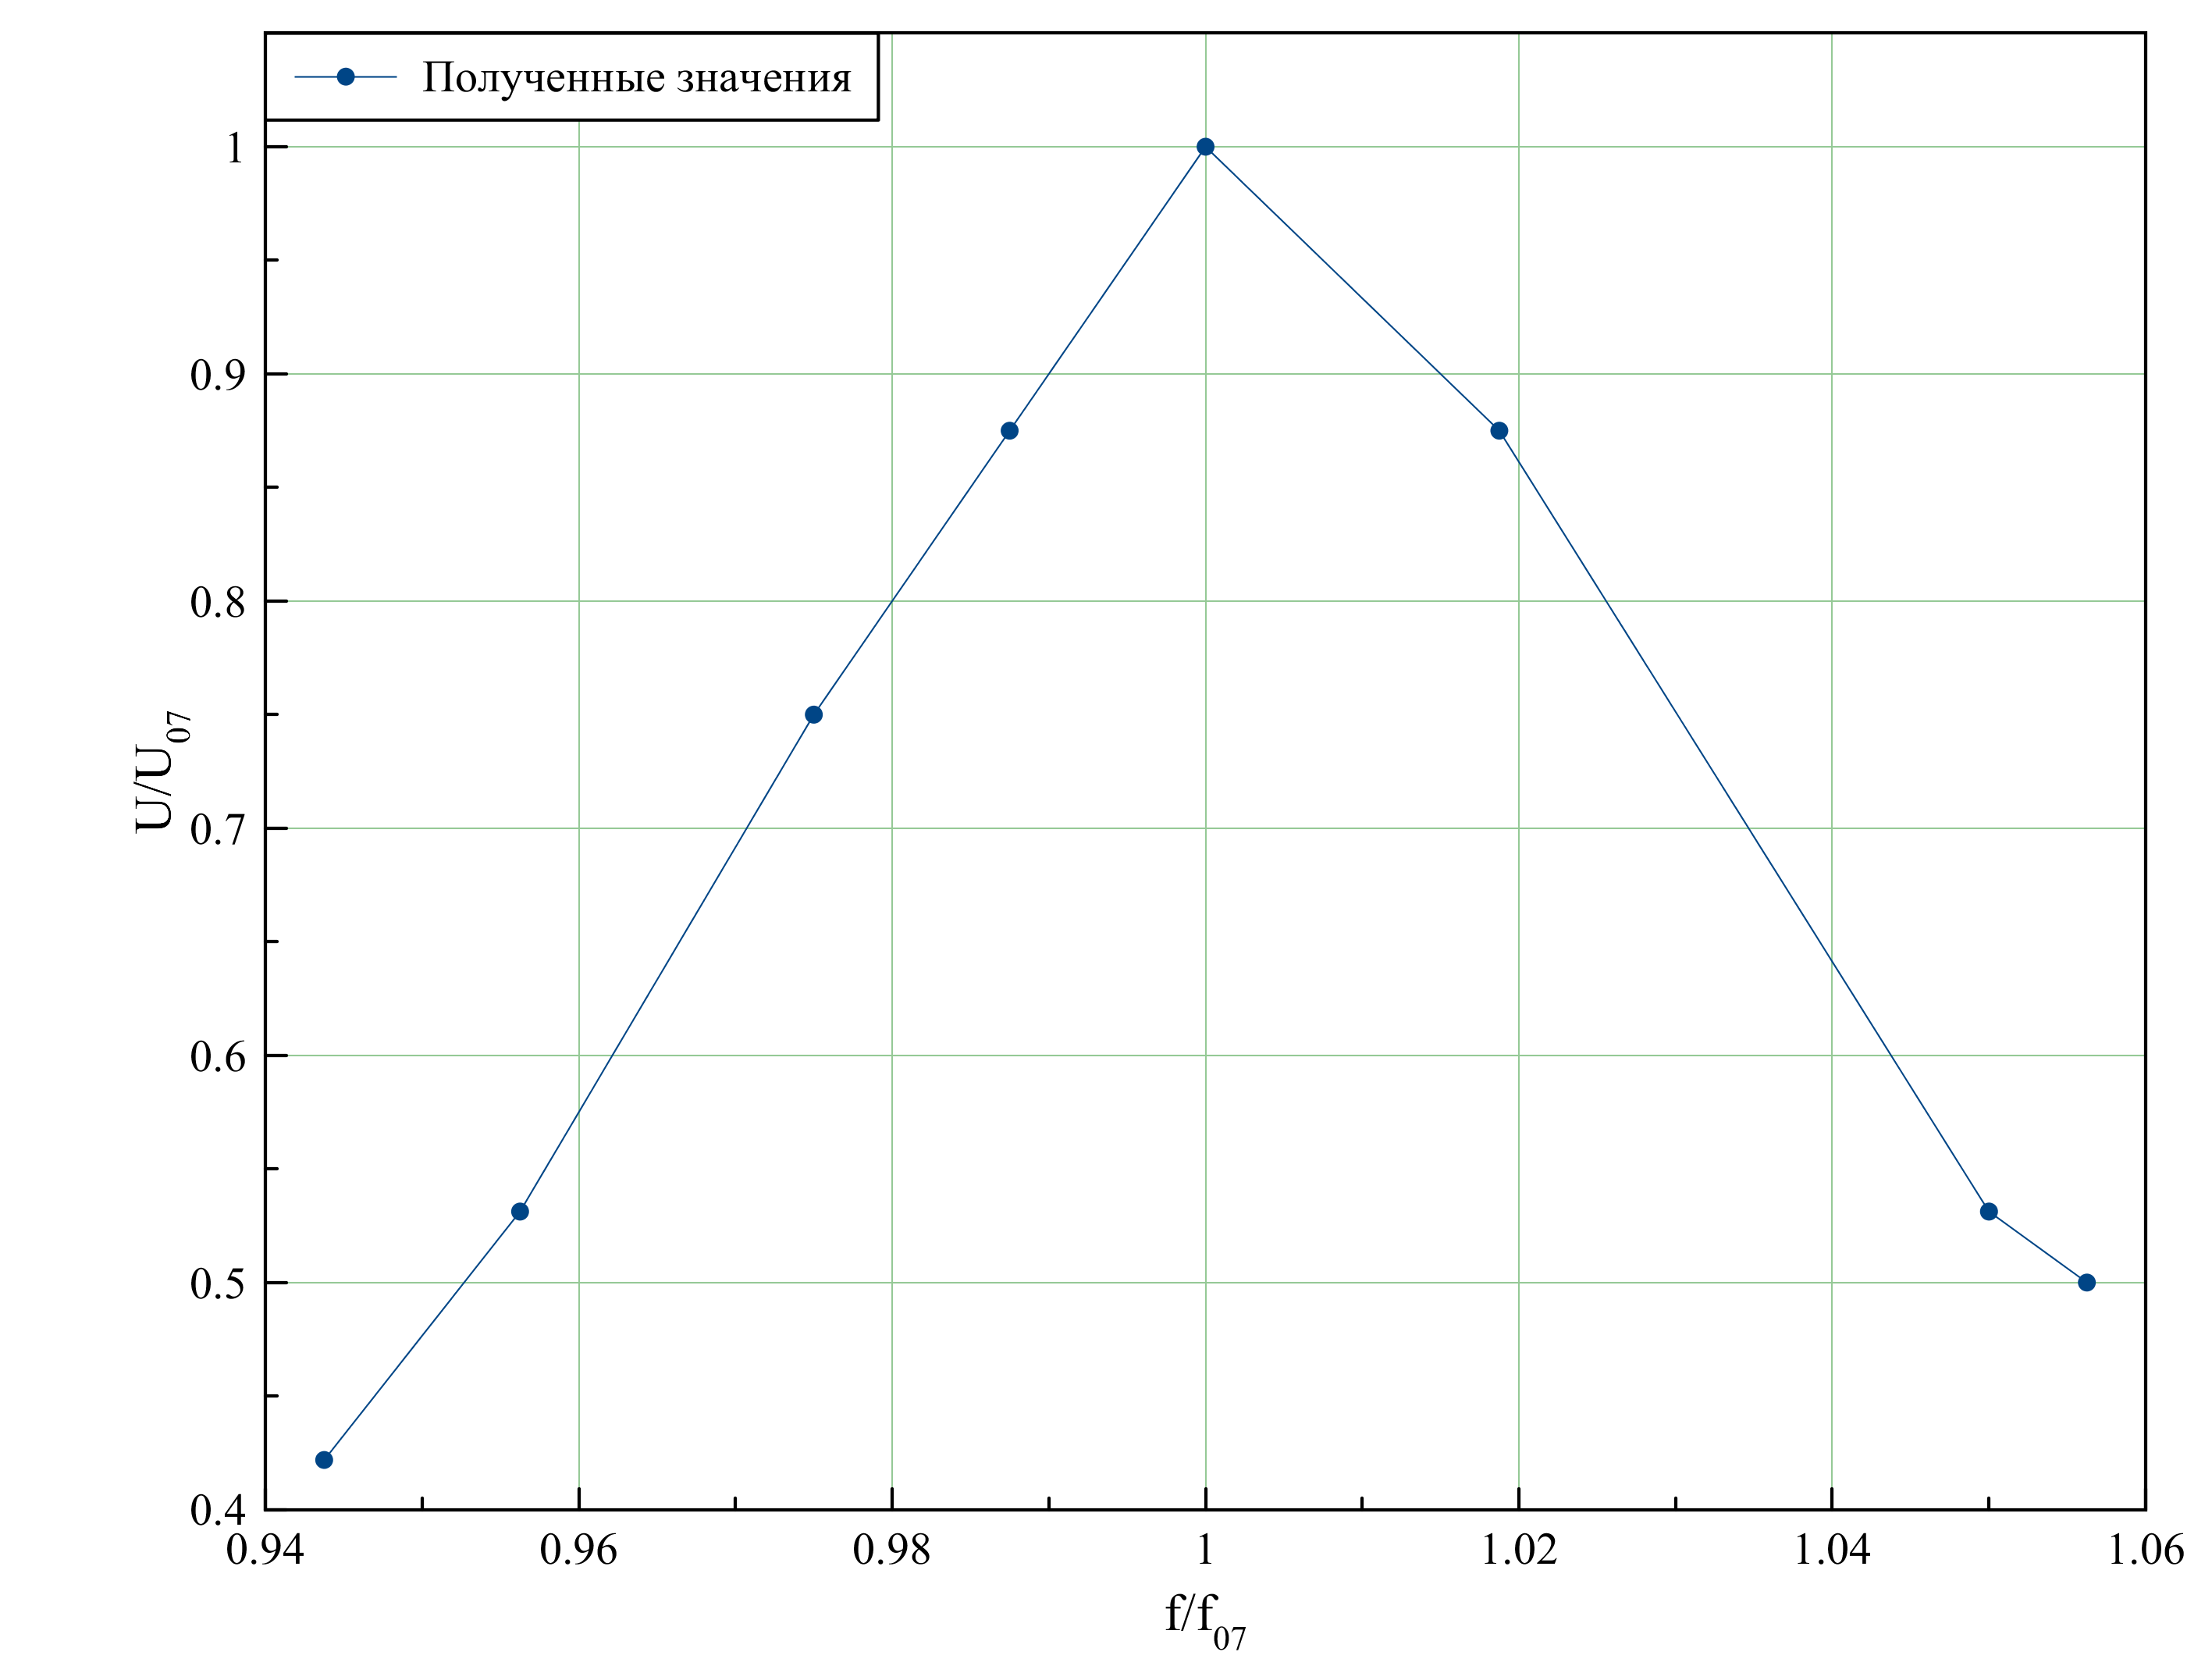
\includegraphics[width=85mm]{2ACH_C7} \\ $C_7$}
	\end{minipage}
	\caption{Амплитудно-частотные характеристики в безразмерных координатах.}
	\label{ris:image3}
\end{figure}
Ширина резонансных кривых на уровне 0.707 для $C_1$ равна 0.03, тогда добротность равна $Q=0.03^{-1}=30.0$\\
Ширина резонансных кривых на уровне 0.707 для $C_7$ равна 0.06, тогда добротность равна $Q=0.06^{-1}=16.7$

Проведем аналогичные действия с ФЧХ для $C_1$ и $C_7$:

\begin{table}[H]
	\centering
	\caption{ФЧХ $C_1$}
	\label{table3.1}
	\begin{tabular}{c|c|c|c|c|c|c|c|c}
		\toprule
		$f$, кГц & 30.4 & 30.9 & 31.3 & 31.8 & 32.5 & 32.9 & 33.2 & 33.4 \\ 
		$f/f_0$ & 0.95 & 0.96 & 0.98  & 0.99  & 1.01 & 1.03 & 1.03 & 1.04 \\ 
		$x_0$ & 1.6 & 1.6 & 1.6 & 1.5 & 0.3 & 0.4 & 0.5 & 0.6 \\ 
		$x$ & 0.9 & 1 & 1 & 1.3 & 1.5 & 1.5 & 1.5 & 1.6 \\ 
		$x/x_0$ & 1.78 & 1.60 & 1.60 & 1.15 & -0.20 & -0.27 & -0.33 & -0.375 \\ \bottomrule
	\end{tabular}
\end{table}

\begin{table}[H]
	\centering
	\caption{ФЧХ $C_7$}
	\label{table3.2}
	\begin{tabular}{c|c|c|c|c|c|c|c|c|c|c|c}
		\toprule
		$f$, кГц & 14.7 & 15 & 15.2 & 15.6 & 15.8 & 16 & 16.3 & 16.6 & 17.2 & 17.4 & 17.6 \\ 
		$f/f_0$ & 0.92 & 0.94 & 0.95 & 0.98 & 0.99 & 1.00 & 1.02 & 1.04 & 1.08 & 1.09 & 1.1 \\ 
		$x_0$ & 3.4 & 3.3 & 3.3 & 3.2 & 3.1 & 3.2 & 0.6 & 0.8 & 1.2 & 1.2 & 1.2 \\ 
		$x$ & 2.1 & 2.1 & 2.2 & 2.4 & 2.6 & 3.2 & 3 & 3 & 2.8 & 2.8 & 2.8 \\ 
		$x/x_0$ & 1.62 & 1.57 & 1.50 & 1.33 & 1.19 & 1 & -0.2 & -0.27 & -0.43 & -0.43 & -0.43 \\ \bottomrule
	\end{tabular}
\end{table}

\begin{figure}[H]
	\begin{minipage}[H]{0.49\linewidth}
		\center{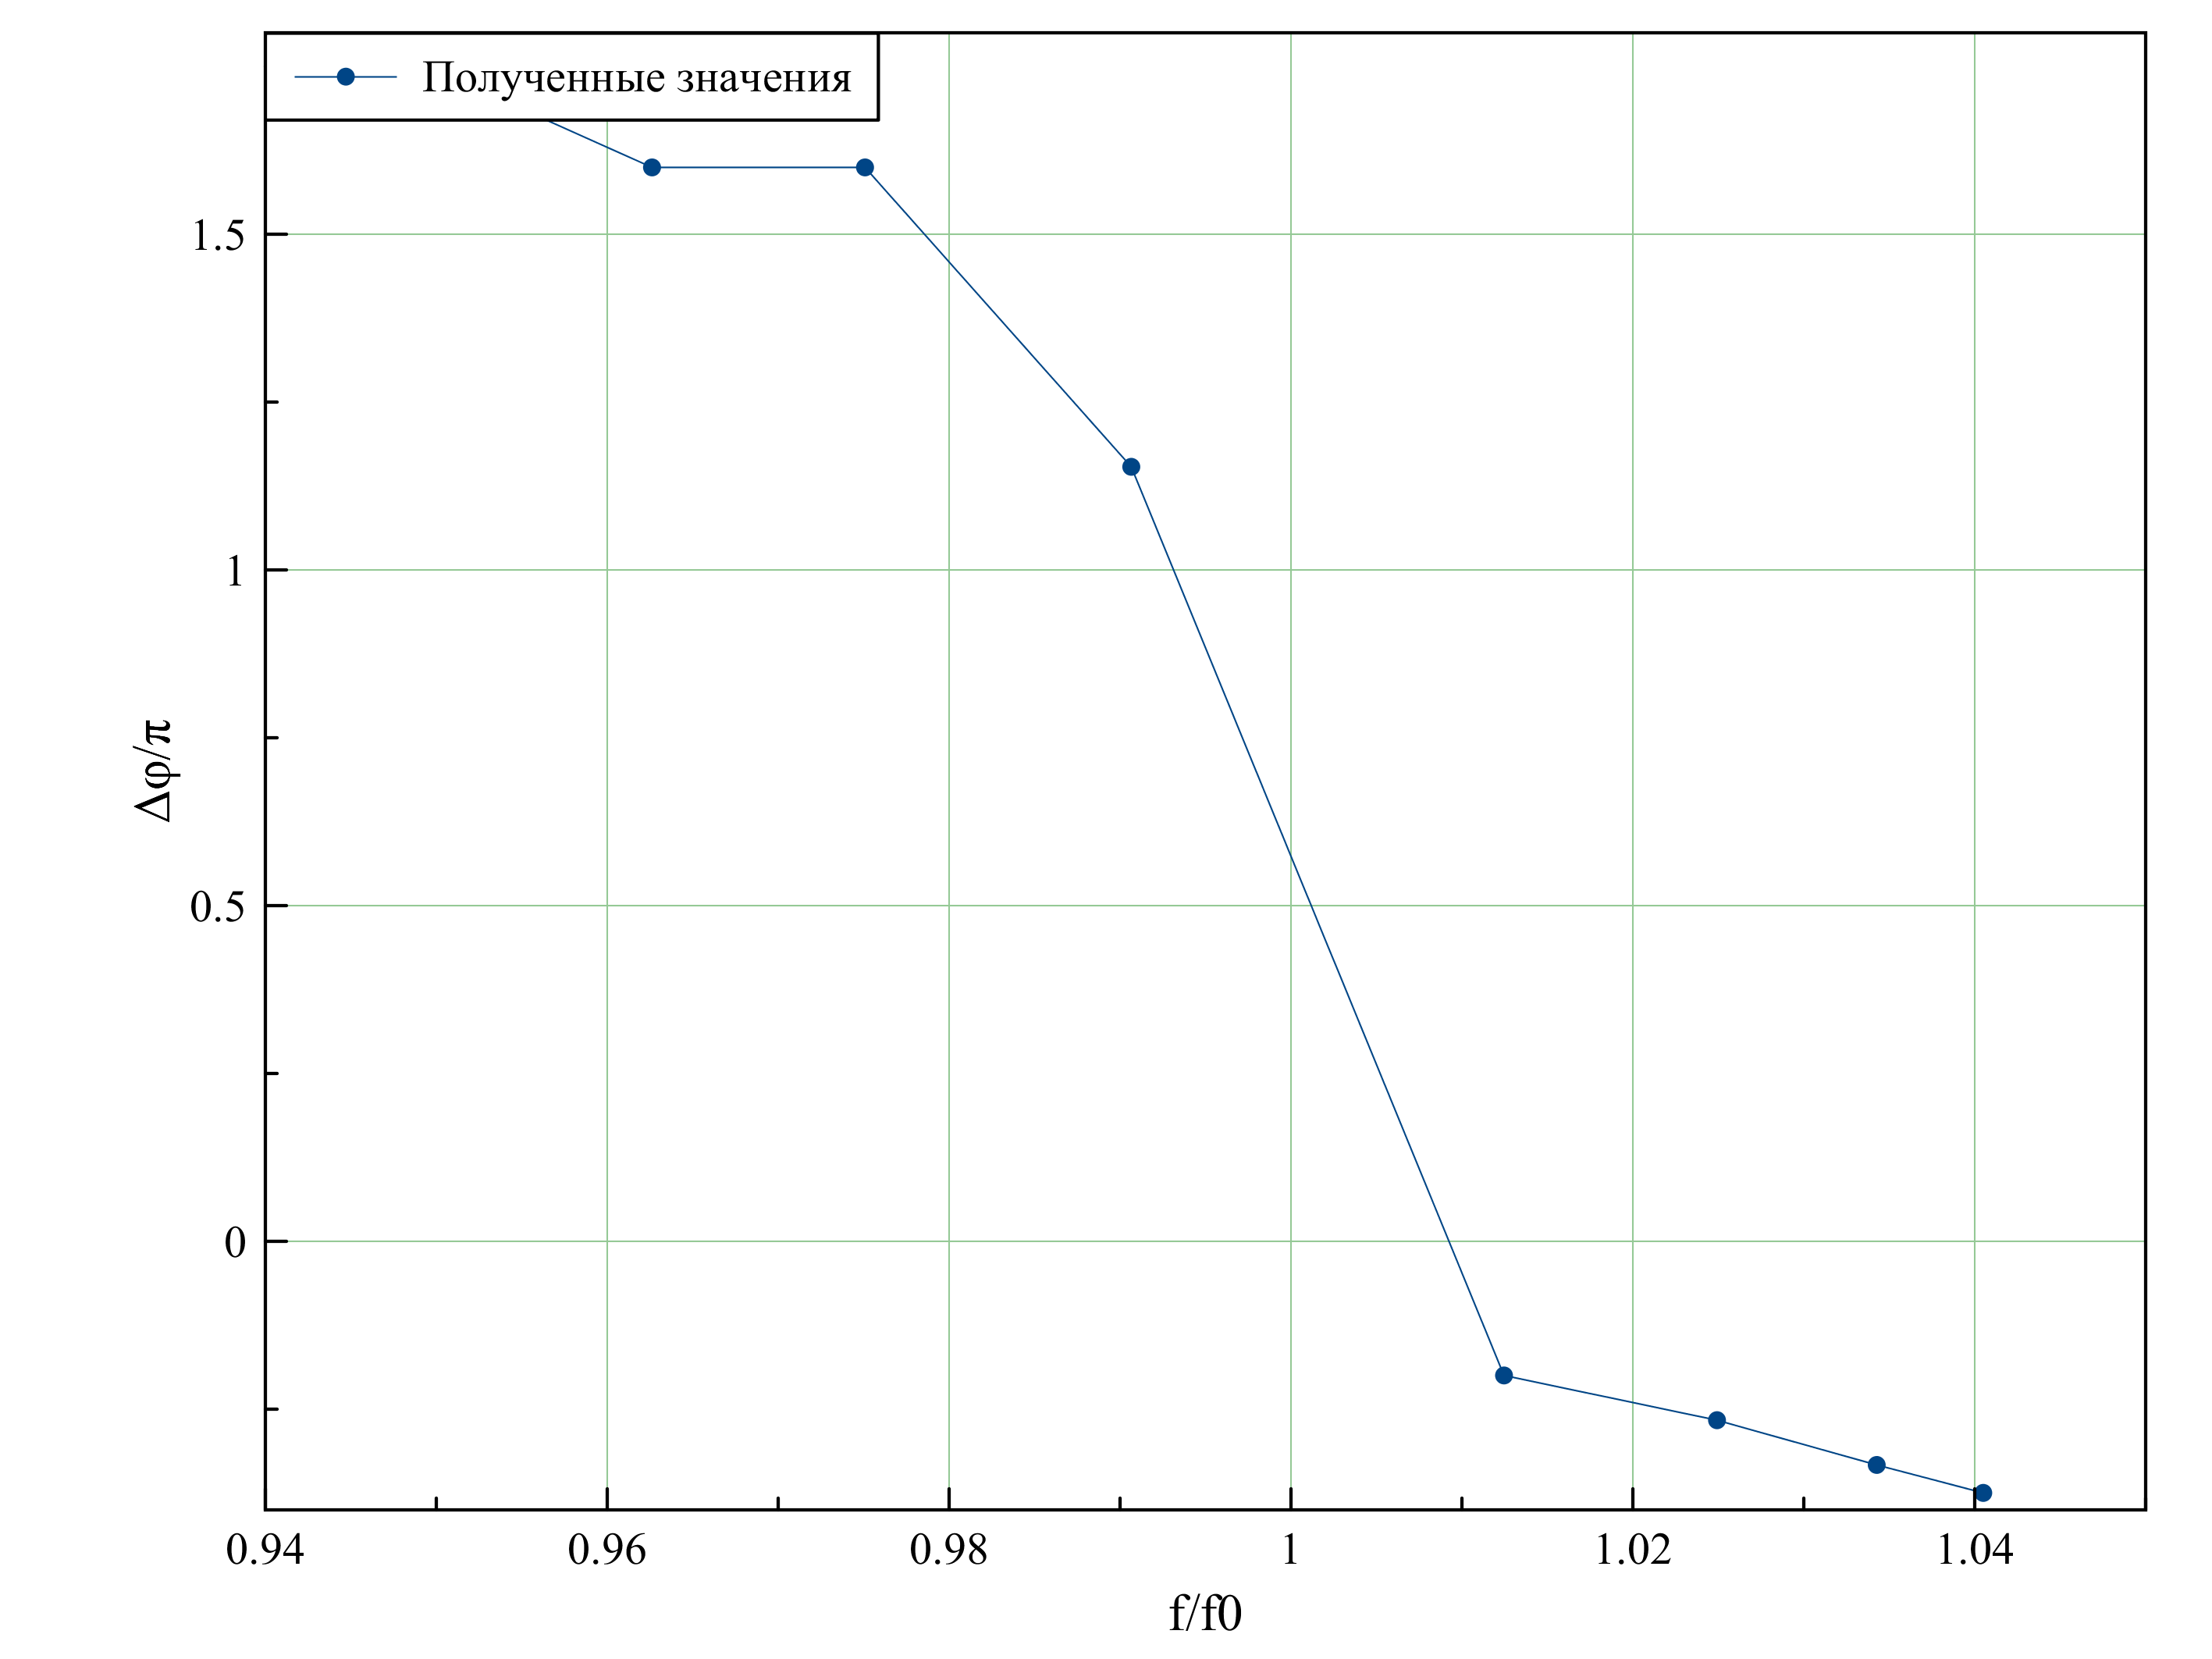
\includegraphics[width=80mm]{FCH_C1} \\ $C_1$}
	\end{minipage}
	~
	\begin{minipage}[h]{0.49\linewidth}
		\center{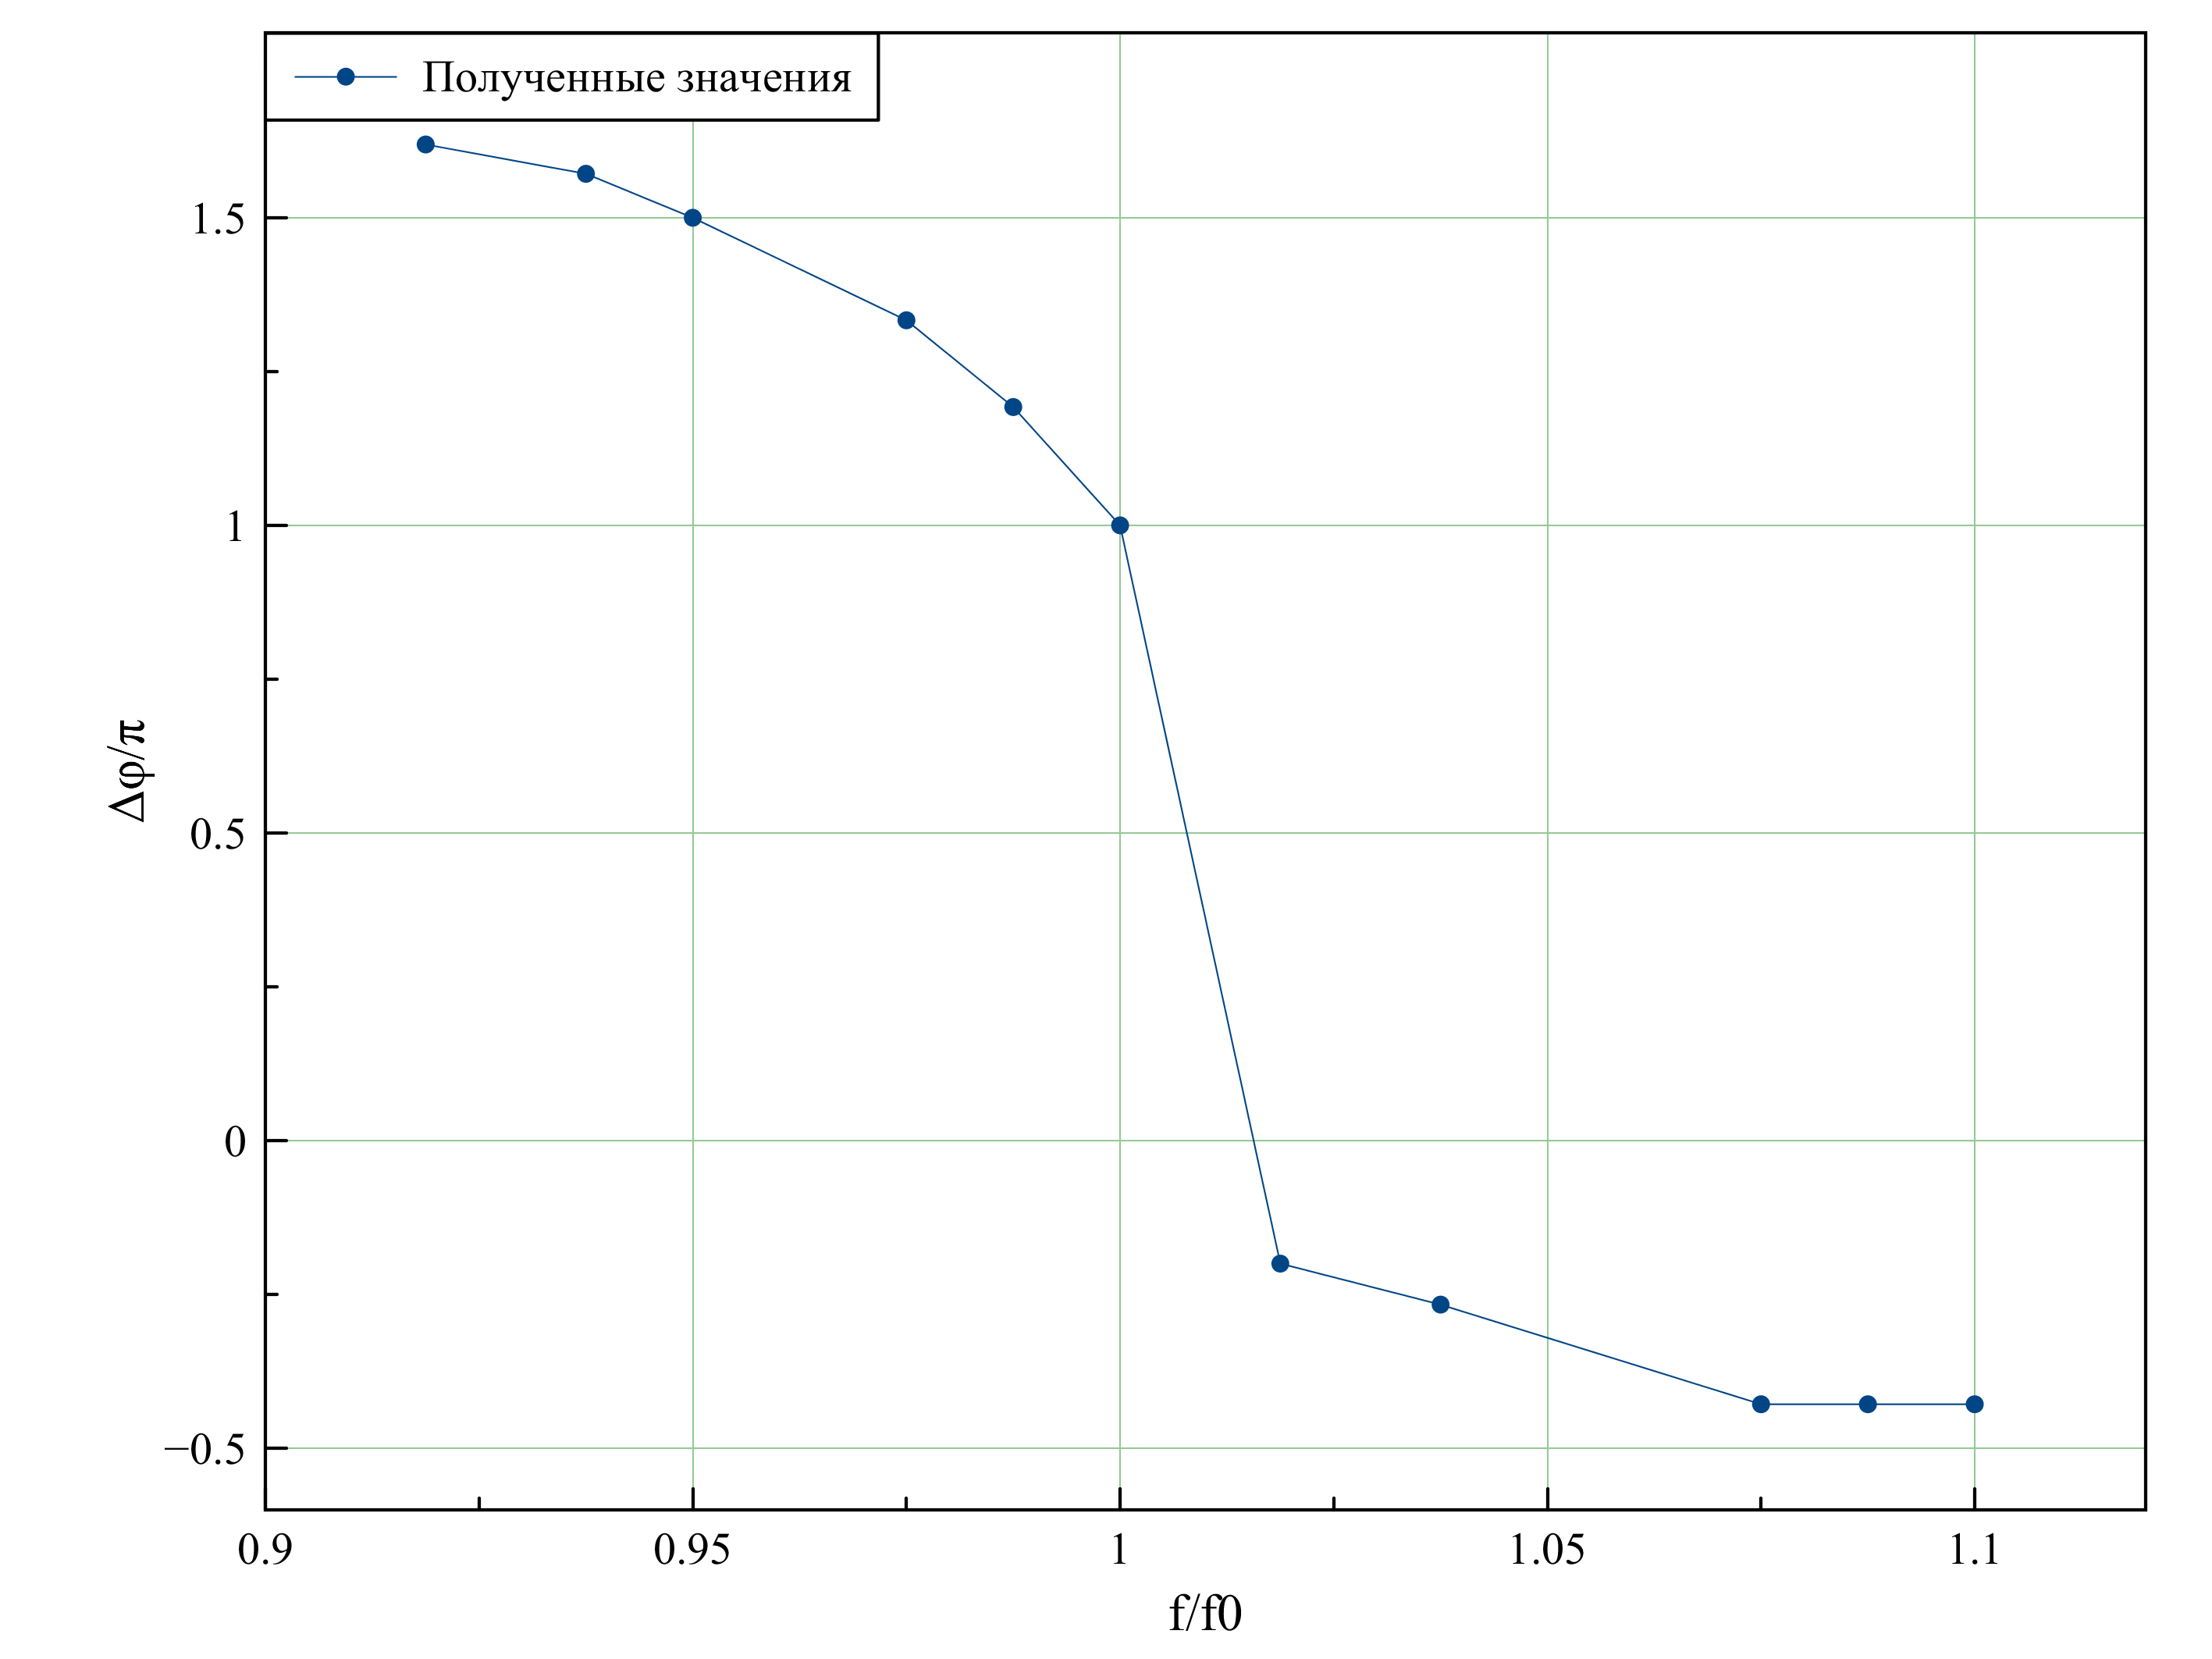
\includegraphics[width=80mm]{FCH_C7} \\ $C_7$}
	\end{minipage}
	\caption{Фазово-частотные характеристики.}
	\label{ris:image4}
\end{figure}
По графикам рассчитаем добротность по расстоянию между точками по оси $x$, в которых y меняется от $\pi/4$ до $-\pi/4$, равному $1/Q$. Для $C_1$ это расстояние равно 0.027, следовательно $Q=36$. Аналогично для $C_7$ $x=0.07$, следовательно $Q=14$. 	

Также отобразим зависимость $R_L$ от $f_{0n}$:

\begin{minipage}[H]{0.49\linewidth}
\begin{figure}[H]
	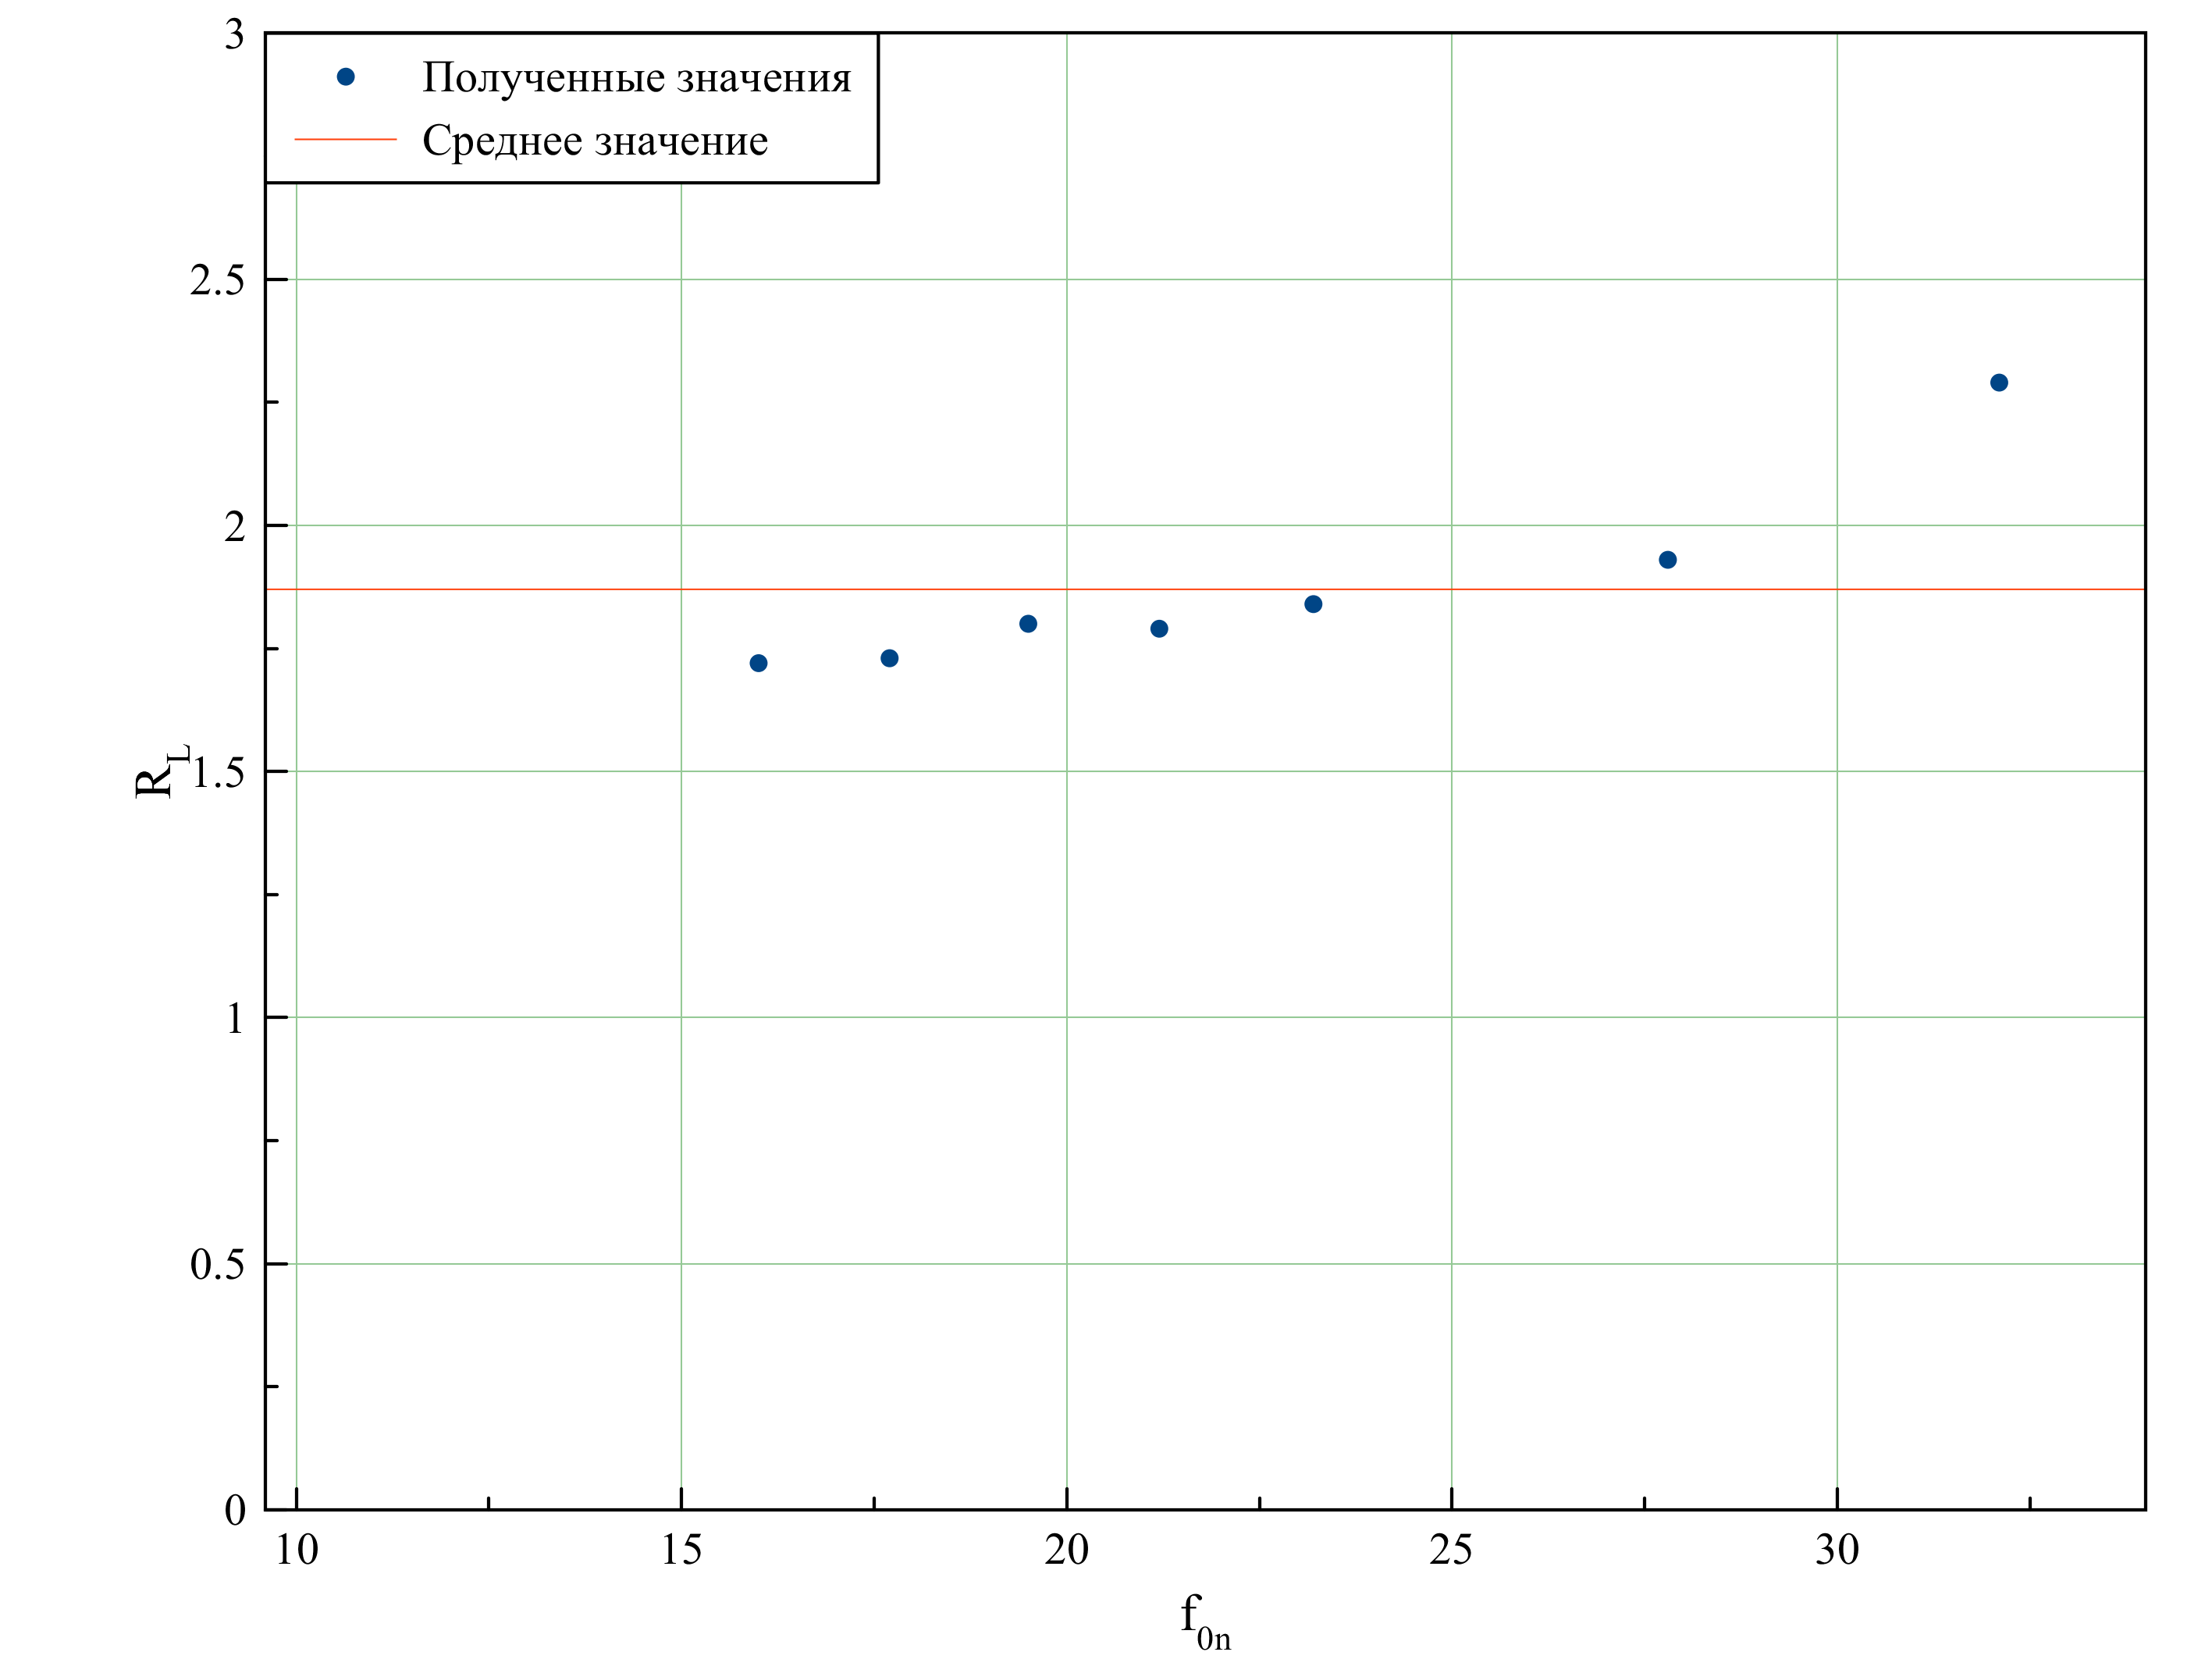
\includegraphics[width=80mm]{RL}
	\caption{Зависимость $R_L$ от $f_{0n}$}
\end{figure}
\end{minipage}
~
\begin{minipage}[H]{0.49\linewidth}
	\textbf{Вывод:} мы исследовали резонанс токов в параллельном колебательном контуре с изменяемой ёмкостью,получили АЧХ и ФЧХ, а также определили основные параметры контура.
\end{minipage}
\end{document}
